\documentclass[11pt]{article}
\usepackage[a4paper,margin=1in]{geometry}
\usepackage{amsmath,amssymb,amsfonts,mathtools,bm}
\usepackage{tikz}
\usetikzlibrary{arrows.meta,positioning}
\usepackage{booktabs}
\usepackage{microtype}
\usepackage{parskip}

\pagestyle{plain}

\newcommand{\R}{\mathbb{R}}
\newcommand{\N}{\mathbb{N}}
\newcommand{\eps}{\varepsilon}
\newcommand{\one}{\mathbf{1}}
\newcommand{\softmax}{\operatorname{softmax}}
\newcommand{\TopK}{\operatorname{TopK}}
\newcommand{\row}{\operatorname{row}}
\newcommand{\norm}[1]{\left\lVert #1 \right\rVert}
\newcommand{\ceil}[1]{\left\lceil #1 \right\rceil}
\newcommand{\floor}[1]{\left\lfloor #1 \right\rfloor}

\title{\textbf{Math-Routed Sparse Transformer}\\[6pt]
\large Architecture Reference}
\author{}
\date{}

\begin{document}
\maketitle

% ─────────────────────────────────────────────────────────────────────────────
\section*{Overview}

The Math-Routed Sparse Transformer compiles mathematical expression structure
into a sparse attention routing table \emph{before} model inference runs.
The central claim is:

\[
\boxed{
  \text{symbolic topology}
  \;\longrightarrow\;
  \text{bounded neural attention}
}
\]

Instead of computing full $O(T^{2})$ dense attention over $T$ tokens,
each token attends only to a fixed-$K$ neighborhood derived from the
mathematical structure of the input expression,
reducing the attention kernel cost to $O(TK)$.

\medskip
All three topology modes (symbolic, learned, block) produce the same
two tensors that feed the Triton sparse attention kernel:

\[
\mathcal{N} \in \mathbb{Z}^{T \times K}
\quad\text{(neighbor index table)},
\qquad
V \in \{0,1\}^{T \times K}
\quad\text{(validity mask)}.
\]

Topology construction is offline.  The compiled $(\mathcal{N}, V)$ pair
is stored as static buffers and reused across all model forwards
without rebuilding.

% ─────────────────────────────────────────────────────────────────────────────
\section*{Notation}

\begin{center}
\begin{tabular}{ll}
\toprule
Symbol & Meaning \\
\midrule
$T$       & number of tokens (math nodes) \\
$d$       & model dimension \\
$d_h$     & head dimension, $d_h = d / H$ \\
$H$       & number of attention heads \\
$K$       & neighbor budget per token \\
$L$       & number of transformer layers \\
$b$       & block size (block topology) \\
$B$       & number of blocks, $B = \ceil{T/b}$ \\
$R$       & number of symbolic relation types \\
$d_E$     & frozen node embedding dimension \\
$d_F$     & learned edge feature dimension \\
\bottomrule
\end{tabular}
\end{center}

% ─────────────────────────────────────────────────────────────────────────────
\section*{Token Representations}

Each math node $i$ is encoded to a frozen embedding $e_i \in \R^{d_E}$
by the \texttt{MathEmbedder}.  These embeddings do not change during
training.  They are used only to build the topology;
the model itself operates on learned projections $x_i \in \R^{d}$.

\subsection*{Direction--Magnitude Decomposition}

The embedding is decomposed into a unit-norm direction and a scalar magnitude:

\[
m_i = \norm{e_i}_2,
\qquad
\hat{e}_i = \frac{e_i}{m_i + \eps},
\qquad
\hat{e}_i \in S^{d_E - 1}.
\]

The unit sphere $S^{d_E - 1} \subset \R^{d_E}$ is
$\{u \in \R^{d_E} : \norm{u}_2 = 1\}$.
Restricting directions to the sphere makes cosine similarity the
natural measure of symbolic alignment:

\[
\cos\theta_{ij} = \hat{e}_i^{\mathsf{T}} \hat{e}_j,
\qquad
\norm{\hat{e}_i - \hat{e}_j}_2^2 = 2(1 - \cos\theta_{ij}).
\]

\begin{center}
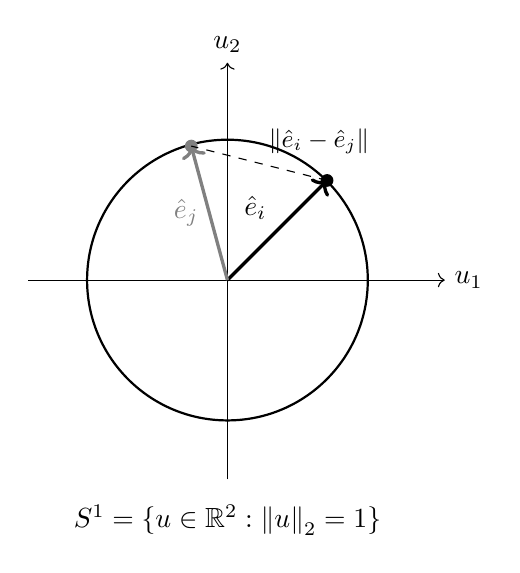
\begin{tikzpicture}[scale=1.15]
  \draw[->] (-2.2,0) -- (2.4,0) node[right] {$u_1$};
  \draw[->] (0,-2.2) -- (0,2.4) node[above] {$u_2$};
  \draw[thick] (0,0) circle (1.55);
  \draw[very thick,->] (0,0) -- (1.10,1.10)
    node[midway,above left] {$\hat{e}_i$};
  \draw[very thick,->,gray] (0,0) -- (-0.40,1.48)
    node[midway,left] {$\hat{e}_j$};
  \fill (1.10,1.10) circle (2pt);
  \fill[gray] (-0.40,1.48) circle (2pt);
  \draw[dashed] (1.10,1.10) -- (-0.40,1.48)
    node[midway,above right,font=\small] {$\norm{\hat{e}_i-\hat{e}_j}$};
  \node at (0,-2.65) {$S^{1}=\{u\in\R^2:\norm{u}_2=1\}$};
\end{tikzpicture}
\end{center}

\subsection*{Projection from Embedding Space to Model Space}

The frozen embeddings live in $\R^{d_E}$; the transformer operates
in $\R^{d}$.  A learned linear projection maps between the two:

\[
x_i^{(0)} = W_{\text{proj}}\, e_i,
\qquad
W_{\text{proj}} \in \R^{d \times d_E}.
\]

For this projection to preserve neighbourhood structure, the
$(\hat{e}_i, \hat{e}_j)$ distances before projection should
approximately equal those after:

\[
(1-\delta)\norm{\hat{e}_i - \hat{e}_j}_2^2
\;\leq\;
\norm{R\hat{e}_i - R\hat{e}_j}_2^2
\;\leq\;
(1+\delta)\norm{\hat{e}_i - \hat{e}_j}_2^2,
\]

which implies:

\[
\hat{e}_i^{\mathsf{T}}\hat{e}_j
\;\approx\;
\hat{z}_i^{\mathsf{T}}\hat{z}_j,
\qquad
z_i = R\hat{e}_i,\quad
\hat{z}_i = \frac{z_i}{\norm{z_i}_2 + \eps}.
\]

\[
\boxed{
  S^{d_E-1}
  \xrightarrow{\;R\;}
  S^{d-1}
  \quad\text{if distances and cosines are preserved within }\delta
}
\]

% ─────────────────────────────────────────────────────────────────────────────
\section*{Symbolic Topology}

The symbolic topology builder constructs a scored graph over the $T$ tokens
by computing $R$ binary relation matrices and combining them with
relation-type weights.  All relation matrices are computed from
the frozen embeddings and the expression structure; none require
a model forward pass.

\subsection*{Relation Types}

Each relation type $r$ defines a binary matrix $M^{(r)} \in \{0,1\}^{T\times T}$:

\medskip
\begin{center}
\begin{tabular}{lp{8cm}}
\toprule
Relation & Definition \\
\midrule
$M^{\text{id}}_{ij}$            & $\mathbf{1}[i=j]$ (self) \\
$M^{\text{dep}}_{ij}$           & $\mathbf{1}[(i,j) \in \text{AST edges}]$ (symbolic dependency) \\
$M^{\text{comp}}_{ij}$          & $\mathbf{1}[j \text{ is a composition argument of } i]$ \\
$M^{\text{shp}}_{ij}$           & $\mathbf{1}[\text{shapes of } i,j \text{ are compatible}]$ \\
$M^{\text{emb}}_{ij}$           & $\mathbf{1}[\hat{e}_i^{\mathsf{T}}\hat{e}_j \geq \tau_{\text{emb}}]$ \\
$M^{\text{win}}_{ij}$           & $\mathbf{1}[|i-j| \leq w]$ (local window) \\
$M^{\text{op}}_{ij}$            & $\mathbf{1}[\text{op}(i) = \text{op}(j)]$ (same operator) \\
$M^{\text{mid}}_{ij}$           & middle-bridge relation (see below) \\
\bottomrule
\end{tabular}
\end{center}

\subsection*{Weighted Priority Score}

Each relation type is assigned a non-negative weight $w_r \geq 0$
and a priority level $p_r \in \mathbb{Z}_{\geq 0}$.
The combined priority score is:

\[
S_{ij}^{\text{sym}}
= \sum_{r=1}^{R} p_r \cdot M^{(r)}_{ij}.
\]

Tokens with higher priority scores are preferred as neighbours.
Ties within the same priority level are broken by the weighted score:

\[
\tilde{S}_{ij}^{\text{sym}}
= \sum_{r=1}^{R} w_r \cdot M^{(r)}_{ij}.
\]

\subsection*{Top-$K$ Neighbour Selection}

For each token $i$, the $K$ highest-scoring column indices are selected:

\[
\mathcal{N}_i^{\text{sym}}
= \TopK_j\!\left(S_{ij}^{\text{sym}},\; K\right),
\qquad
|\mathcal{N}_i^{\text{sym}}| = K.
\]

The resulting table $\mathcal{N}^{\text{sym}} \in \mathbb{Z}^{T\times K}$
and validity mask $V^{\text{sym}} \in \{0,1\}^{T\times K}$
are cached.  No $O(T^2)$ mask is materialised at inference time.

% ─────────────────────────────────────────────────────────────────────────────
\section*{Middle-Preserving Topology (v7)}

Standard top-$K$ selection tends to concentrate neighbours near
the sequence endpoints and the root.  Tokens in the middle of a long
expression are under-represented — the ``lost-in-the-middle'' problem.

The middle-bridge relation explicitly connects each token to a window
of $w$ tokens centred on the midpoint $T/2$:

\[
M^{\text{mid}}_{ij}
=
\mathbf{1}\!\left[\left|j - \tfrac{T}{2}\right| \leq w\right].
\]

This relation is included in the scored top-$K$ build with
weight $w_{\text{mid}} = 0.7$ and priority $p_{\text{mid}} = 4$.
The combined score becomes:

\[
S_{ij}
= \alpha \cdot M^{\text{id}}_{ij}
+ \sum_{r \neq \text{mid}} \beta_r M^{(r)}_{ij}
+ \gamma \cdot M^{\text{mid}}_{ij}.
\]

Because the top-$K$ selection is applied to $S_{ij}$ directly,
the resulting topology is fixed-$K$ by construction:

\[
|\mathcal{N}_i| = K \quad \forall\; i,
\qquad \text{(no runtime truncation needed)}.
\]

At $T=1024$, $K=16$, trees mode, the middle-bridge topology produces:

\[
\text{allowed edges} = T \cdot K = 16{,}384
\qquad\text{vs}\qquad
\text{full} = T^2 = 1{,}048{,}576.
\]

% ─────────────────────────────────────────────────────────────────────────────
\section*{Learned Topology}

The symbolic topology encodes hand-crafted rules.
Learned topology replaces the scoring function with a neural network
trained to select neighbours that maximise route quality.

\subsection*{Edge Feature Tensor}

For each token pair $(i,j)$, a feature vector is computed from the
frozen embeddings and symbolic relation matrices:

\[
F_{ij} =
\bigl[
  M^{\text{id}}_{ij},\;
  M^{\text{dep}}_{ij},\;
  M^{\text{comp}}_{ij},\;
  M^{\text{shp}}_{ij},\;
  M^{\text{mid}}_{ij},\;
  M^{\text{win}}_{ij},\;
  M^{\text{op}}_{ij},\;
  \hat{e}_i^{\mathsf{T}}\hat{e}_j,\;
  \tfrac{|i-j|}{T},\;
  \tfrac{i-j}{T}
\bigr]^{\mathsf{T}}
\in \R^{d_F},
\]

with $d_F = 10$.  The full edge feature tensor is
$F \in \R^{T \times T \times d_F}$.

\subsection*{Scorer}

A learned scorer maps each edge feature to a scalar score:

\[
S_{ij}^{\text{learned}} = f_\theta(F_{ij}) \in \R.
\]

Top-$K$ neighbour selection proceeds identically to the symbolic case:

\[
\mathcal{N}_i^{\text{learned}}
= \TopK_j\!\left(S_{ij}^{\text{learned}},\; K\right).
\]

\subsection*{Scaling Limitation}

Building $F$ requires computing all $T^2$ token pairs.
The scoring cost is:

\[
\text{cost} = O(T^2 \cdot d_F).
\]

For $T = 4096$: $T^2 = 16{,}777{,}216$ pairs --- this causes an
out-of-memory error during topology construction.
The block topology (below) resolves this.

\medskip
\textbf{Empirical result.}  On \texttt{synthetic\_hard/val.jsonl}:

\[
Q_{\text{learned},\,K=6} = 0.9871
\quad>\quad
Q_{\text{hand},\,K=16} = 0.9821.
\]

The learned scorer achieves higher route accuracy at a smaller
neighbour budget than the hand-designed symbolic topology.

% ─────────────────────────────────────────────────────────────────────────────
\section*{Block Topology (v14)}

Block topology replaces token-pair scoring with block-pair scoring,
reducing the quadratic cost by a factor of $b^2$.

\subsection*{Block Partition}

The $T$ tokens are divided into $B$ contiguous blocks of size $b$:

\[
B = \ceil{T/b},
\qquad
\text{block } \beta = \{(\beta-1)b,\; \ldots,\; \min(\beta b,\, T) - 1\}.
\]

\subsection*{Block Features}

Each block $\beta$ is summarised by a feature vector $\phi_\beta \in \R^{d_B}$
computed from the operator histogram, node-kind histogram, shape summary,
and middle-token coverage of the tokens it contains.

\subsection*{Block Scoring}

Block pairs are scored with a heuristic function:

\[
S_{\beta\gamma}^{\text{block}}
= S_{\text{local}}(\beta,\gamma)
+ S_{\text{bridge}}(\beta,\gamma)
+ S_{\text{mid}}(\beta,\gamma)
- \lambda_d \cdot |\beta - \gamma|.
\]

The cost of scoring all block pairs is:

\[
O(B^2) = O\!\left(\frac{T^2}{b^2}\right),
\]

a factor of $b^2$ cheaper than token-pair scoring.
For $T=4096$ and $b=64$: $B^2 = 4{,}096$ vs $T^2 = 16{,}777{,}216$.

\subsection*{Token Expansion}

The top-$K_B$ block neighbours of each block are selected:

\[
\mathcal{N}_\beta^{\text{block}}
= \TopK_\gamma\!\left(S_{\beta\gamma}^{\text{block}},\; K_B\right).
\]

Each token $i$ in block $\beta$ inherits the token ranges of all
selected neighbouring blocks:

\[
\mathcal{N}_i^{\text{token}}
= \bigcup_{\gamma\,\in\,\mathcal{N}_{\beta(i)}^{\text{block}}}
  \bigl\{\, t \;:\; \gamma b \leq t < \min\bigl((\gamma+1)b,\, T\bigr) \bigr\}.
\]

This is capped to $K$ tokens per row (matching the fixed-$K$ interface
of the other topology modes), with local-window and symbolic-bridge
tokens added:

\[
\mathcal{N}_i^{\text{final}}
= \TopK\!\left(
    \mathcal{N}_i^{\text{token}}
    \cup \mathcal{N}_i^{\text{local}}
    \cup \mathcal{N}_i^{\text{bridge}},\;
    K
  \right).
\]

\[
\boxed{
  O(B^2) = O\!\left(\frac{T^2}{b^2}\right)
  \;\longrightarrow\;
  \text{no OOM at }T \in \{1024,\,2048,\,4096\}
}
\]

% ─────────────────────────────────────────────────────────────────────────────
\section*{Sparse Attention Kernel}

All three topology modes produce the same interface.
The Triton sparse attention kernel consumes the neighbor table directly,
without materialising an $O(T^2)$ attention matrix.

\subsection*{Projections}

For layer $\ell$ and head $h$, the input $X^{(\ell)} \in \R^{T \times d}$
is projected to queries, keys, and values:

\[
Q^{(\ell,h)} = X^{(\ell)} W_Q^{(\ell,h)},
\quad
K^{(\ell,h)} = X^{(\ell)} W_K^{(\ell,h)},
\quad
V^{(\ell,h)} = X^{(\ell)} W_V^{(\ell,h)},
\]

\[
W_Q^{(\ell,h)},\, W_K^{(\ell,h)},\, W_V^{(\ell,h)} \in \R^{d \times d_h}.
\]

\subsection*{Neighbour-Sparse Attention}

For each token $i$, attention is computed only over its $K$ neighbours.
Let $\mathcal{N}_{i,k}$ denote the $k$-th neighbour index of token $i$.
The raw attention scores are:

\[
a_{i,k}^{(\ell,h)}
= \frac{q_i^{(\ell,h)\mathsf{T}} k_{\mathcal{N}_{i,k}}^{(\ell,h)}}{\sqrt{d_h}},
\qquad k = 1,\ldots,K.
\]

Valid neighbours are selected by the mask $V_{i,k} \in \{0,1\}$:

\[
p_{i,k}^{(\ell,h)}
= \frac{V_{i,k}\exp(a_{i,k}^{(\ell,h)})}
       {\sum_{k'=1}^{K} V_{i,k'}\exp(a_{i,k'}^{(\ell,h)})}.
\]

The output for token $i$ is the weighted sum over neighbour values:

\[
o_i^{(\ell,h)}
= \sum_{k=1}^{K} p_{i,k}^{(\ell,h)}\; v_{\mathcal{N}_{i,k}}^{(\ell,h)}.
\]

\subsection*{Multi-Head Concatenation and Output Projection}

The per-head outputs are concatenated and projected:

\[
O^{(\ell)}
= \bigl[o^{(\ell,1)} \;\cdots\; o^{(\ell,H)}\bigr]\, W_O^{(\ell)},
\qquad W_O^{(\ell)} \in \R^{Hd_h \times d}.
\]

\subsection*{Complexity}

\[
\text{Neighbour-sparse attention: } O(T \cdot K \cdot d_h)
\qquad\text{vs}\qquad
\text{Dense attention: } O(T^2 \cdot d_h).
\]

At $T=1024$, $K=16$, $d_h=32$: the Triton sparse kernel runs at
approximately $0.30\,\text{ms}$ versus $1.96\,\text{ms}$ for dense
attention --- a $6.5\times$ kernel-level speedup.

\subsection*{Block-Token Launch Pattern}

The default Triton kernel uses a block-token program partition:
one Triton program handles $t_{\text{block}}=2$ consecutive token rows
at once (default \texttt{block\_t=2}).  This increases arithmetic
intensity per program launch:

\[
\text{programs} = \frac{T}{t_{\text{block}}} \cdot H \cdot B_{\text{batch}}
\quad\text{vs}\quad
T \cdot H \cdot B_{\text{batch}}
\;\text{ for the one-token variant}.
\]

% ─────────────────────────────────────────────────────────────────────────────
\section*{Transformer Block}

Each transformer layer applies pre-norm attention followed by
a feed-forward network, with residual connections.

\subsection*{Pre-Norm Attention}

\[
\tilde{x}_i^{(\ell)} = \text{LayerNorm}(x_i^{(\ell)}),
\]

\[
x_i^{(\ell+1/2)}
= x_i^{(\ell)}
+ \text{Dropout}\!\left(o_i^{(\ell)}\right),
\qquad
o_i^{(\ell)} = \sum_h W_O^{(\ell)} [o_i^{(\ell,1)}\cdots o_i^{(\ell,H)}]^{\mathsf{T}}.
\]

\subsection*{Feed-Forward Network}

\[
\text{FFN}(x) = W_2\,\text{GELU}(W_1 x + b_1) + b_2,
\qquad
W_1 \in \R^{d_{\text{ff}} \times d},\;
W_2 \in \R^{d \times d_{\text{ff}}}.
\]

\[
x_i^{(\ell+1)}
= x_i^{(\ell+1/2)}
+ \text{Dropout}\!\left(
    \text{FFN}\bigl(\text{LayerNorm}(x_i^{(\ell+1/2)})\bigr)
  \right).
\]

\subsection*{Block Output}

The full block map for layer $\ell$:

\[
\mathcal{B}^{(\ell)}: X^{(\ell)},\,\mathcal{N},\,V
\;\longmapsto\;
X^{(\ell+1)}.
\]

The composed model with $L$ layers:

\[
\mathcal{A}_{\Theta,\mathcal{N},V}
=
\mathcal{B}^{(L-1)} \circ \cdots \circ \mathcal{B}^{(0)} \circ W_{\text{proj}}.
\]

% ─────────────────────────────────────────────────────────────────────────────
\section*{Two-Stage Inference}

Topology construction is too expensive to run in every forward pass.
At $T=1024$, symbolic topology build takes $1$--$2$ seconds.
The architecture is therefore strictly two-stage:

\[
\underbrace{
  \text{nodes}
  \;\longrightarrow\;
  \mathcal{N},\, V
}_{\text{Stage 1: offline compile (once)}}
\qquad\longrightarrow\qquad
\underbrace{
  X^{(0)},\,\mathcal{N},\,V
  \;\longrightarrow\;
  Y
}_{\text{Stage 2: inference (many times)}}.
\]

After \texttt{prepare\_static\_topology} is called, $\mathcal{N}$ and $V$
are stored as registered CUDA buffers.  Every subsequent forward uses
\texttt{forward\_static\_fast\_path}, which reads directly from the
buffers without any topology lookup:

\[
\boxed{
  \text{Stage 2 cost} = O(T \cdot K \cdot d_h \cdot H \cdot L)
  \quad\text{(no topology construction)}
}
\]

% ─────────────────────────────────────────────────────────────────────────────
\section*{Training Objectives}

\subsection*{Route Classification Loss}

The model is trained to predict which expert $y \in \{1,\ldots,E\}$
should handle a given math expression.
The route logit is computed from the root token:

\[
\ell_{\text{route}}(x) = W_{\text{route}}\, x_{0}^{(L)} \in \R^E.
\]

The training loss is cross-entropy:

\[
\mathcal{L}_{\text{route}}
= -\sum_{(x,y) \in \mathcal{D}} \log p_\Theta(y \mid x),
\qquad
p_\Theta(y \mid x) = \softmax(\ell_{\text{route}}(x))_y.
\]

\subsection*{Topology Scorer Loss}

The learned topology scorer is trained with a combined loss:

\[
\mathcal{L}_{\text{scorer}}
= \mathcal{L}_{\text{route}}
+ \lambda_{\text{t}}\,\mathcal{L}_{\text{teacher}}
+ \lambda_{\text{s}}\,\mathcal{L}_{\text{sparsity}},
\]

where the teacher agreement term penalises divergence from the
dense-attention probability distribution $P^{\text{dense}}$:

\[
\mathcal{L}_{\text{teacher}}
= \frac{1}{T}\sum_{i=1}^{T}
  \text{KL}\!\left(P_i^{\text{dense}} \;\Big\|\; P_i^{\text{sparse},K}\right),
\]

and the sparsity term encourages smaller $K$:

\[
\mathcal{L}_{\text{sparsity}}
= \frac{1}{T}\sum_{i=1}^{T} \left|\mathcal{N}_i\right|.
\]

\subsection*{Route Quality Metric}

The primary evaluation metric is route accuracy under sparse attention:

\[
Q(K)
= \frac{1}{|\mathcal{D}|}
  \sum_{(x,y)\in\mathcal{D}}
  \mathbf{1}\!\left[\hat{y}_{\text{sparse},K}(x) = y\right].
\]

Dense agreement measures whether sparse routing produces the same
decision as full attention on the same checkpoint weights:

\[
Q_{\text{agree}}(K)
= \frac{1}{|\mathcal{D}|}
  \sum_{(x,y)\in\mathcal{D}}
  \mathbf{1}\!\left[\hat{y}_{\text{sparse},K}(x) = \hat{y}_{\text{dense}}(x)\right].
\]

The v7 checkpoint achieves $Q_{\text{agree}}(16) = 1.0000$ on the
current synthetic validation split.

\subsection*{Parameter Update}

\[
\Theta_{t+1} = \Theta_t - \eta\,\nabla_\Theta\,\mathcal{L}.
\]

% ─────────────────────────────────────────────────────────────────────────────
\section*{Proven Results}

\begin{center}
\begin{tabular}{lrr}
\toprule
Measurement & Value & Config \\
\midrule
Dense attention          & $1.96\,\text{ms}$  & $T=1024$, trees \\
Triton sparse attention  & $0.30\,\text{ms}$  & $T=1024$, $K=16$, trees \\
Kernel speedup           & $6.5\times$        & \\
\midrule
Dense transformer block  & $2.398\,\text{ms}$ & $T=1024$, $K=16$, trees \\
Cached sparse block      & $2.017\,\text{ms}$ & \\
Prepared static block    & $0.941\,\text{ms}$ & \\
Prepared vs dense speedup & $2.55\times$      & \\
\midrule
Learned $K=6$ route acc  & $0.9871$           & \texttt{synthetic\_hard} \\
Hand $K=16$ route acc    & $0.9821$           & \texttt{synthetic\_hard} \\
\midrule
v7 $Q(K{=}16)$           & $1.0000$           & synthetic val \\
v7 $Q_{\text{agree}}(16)$& $1.0000$           & synthetic val \\
\midrule
Block topology OOM at $T=4096$ & none & $b=64$, $B^2=4{,}096$ \\
Token-pair OOM at $T=4096$     & yes  & $T^2=16{,}777{,}216$ \\
\bottomrule
\end{tabular}
\end{center}

\bigskip

The prepared-static block parity threshold has been crossed:

\[
\boxed{
  p_{\text{blk}} = 0.941\,\text{ms}
  \;<\;
  d_{\text{blk}} = 2.398\,\text{ms}
  \qquad
  (T=1024,\; K=16,\; \text{trees})
}
\]

The remaining overhead distribution within the prepared block:

\[
\frac{p_{\text{attn}}}{p_{\text{blk}}} \approx 34\%
\quad\text{(attention kernel)},
\qquad
\frac{p_{\text{non}}}{p_{\text{blk}}} \approx 66\%
\quad\text{(LayerNorm, QKV, out\_proj, FFN)}.
\]

The bottleneck has shifted from topology construction to
standard transformer block infrastructure.

\end{document}
